\chapter{CMS Trigger System}

When operating at nominal luminosity the LHC produces over 1 billion proton-proton collisions per second.  Finite computing speed and storage capacity limit the rate at which CMS can record events to be about 1 kHz \cite{Cadamuro:2017slr}.  Decreasing the rate from 1 GHz to 1 kHz is accomplished by using a two-level trigger system to quickly decide which events will be discarded and which will be recorded. The first stage is a hardware-based Level 1 (L1) trigger and the second stage is software-based High Level Trigger (HLT).  

\section{L1 trigger}
The L1 trigger decreases the rate by about six orders of magnitude from 1 GHz to 100 kHz by performing rough calculations on information from the ECAL, HCAL, and muon subsystems using field-programmable gate arrays (FPGAs).  The L1 trigger can be divided further into the calorimeter and muon triggers.  The schematic of the L1 trigger system in Figure \ref{fig:l1trigger} shows both the calorimeter and muon triggers.  The calorimeter trigger trigger uses information from the ECAL and HCAL subdetectors to construct photon, electron, and jet candidates in addition to quantities such as missing transverse momentum and total hadronic activity.  The muon trigger uses information from all three muon subsystems to construct muon candidates.  The outputs from the calorimeter and muon triggers goes into the Global Trigger (GT) which decides which events should be recorded and which are to be discarded \cite{Wittmann_2016}.

\begin{figure}
	\centering
	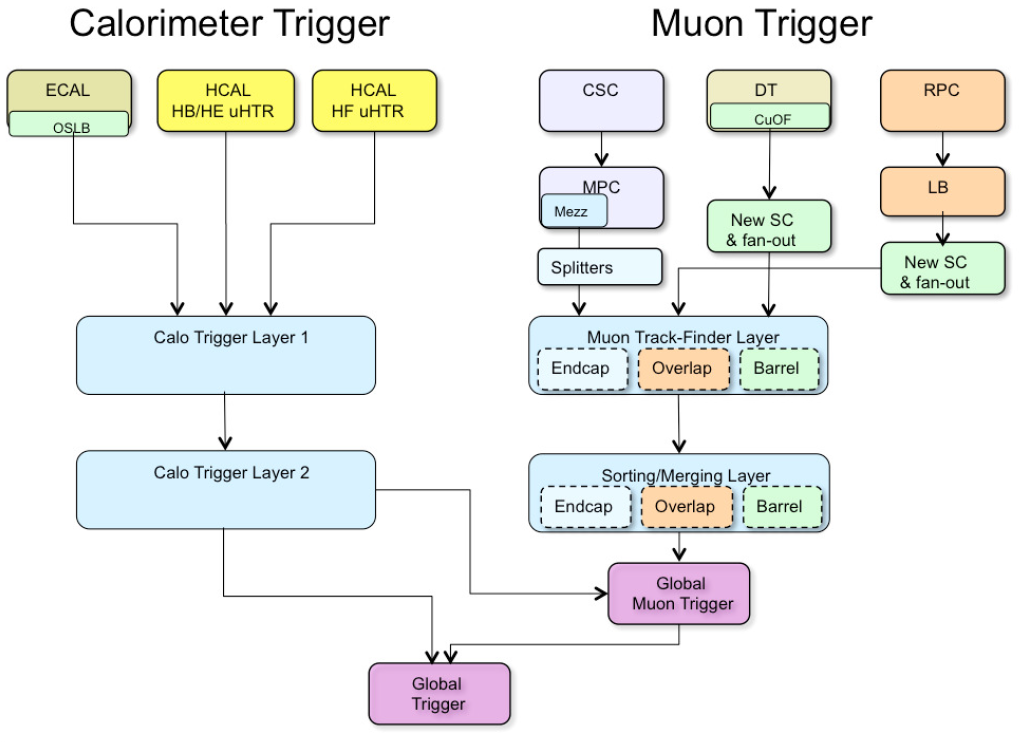
\includegraphics[width=0.9\linewidth]{Figures/L1Trigger}
	\caption{L1 trigger system.  Reprint from \cite{L1Triggerfigure:2013yva}}
	\label{fig:l1trigger}
\end{figure}

\subsection{Calorimeter trigger}
Trigger Primitives (TP) are the raw inputs from the ECAL and HCAL for the calorimeter trigger.  The TP, which contain information regarding the energy deposits in the calorimeters, are passed to the first layer of the calorimeter trigger.  This first layer consists of several FPGA cards that receive data from several bunch crossings, but are each mapped to a section of the detector.  This data is then passed on to the second layer in such a way that each FPGA in this layer will receive data for the entire calorimeter for each bunch crossing.  Candidate objects are then constructed and organized into a sorted list according to transverse momentum and passed on to the GT and the global muon trigger.


\subsection{Muon trigger}
TP for the muon trigger come from the three muon detectors, the CSCs, DTs, and RPCs.  These are then passed on to the first layer of the muon trigger (Muon Track-Finding Layer) where the TP are combined to reconstruct muon tracks for sections of $\phi$ for different regions of $|\eta|$.  The barrel track-finder for $|\eta|<0.83$, the endcap track-finder for $|\eta|>1.24$, and the overlap track-finder for $0.83<|\eta|<1.24$.  This data is passed on to the second layer where the sections of $\phi$ are merged and subsequently passed on to the global muon trigger where it is combined with the output from Calo Trigger Layer 2 to compute isolation.  The global muon trigger then combines the $\eta$ regions and passes a list of the top eight muon candidates to the GT.

\subsection{Global Trigger}
Final processing of the reconstructed objects and quantities constructed by the calorimeter and muon triggers is carried out by the GT.  L1 algorithms or "seeds" are implemented by the GT using these objects.  A full set of L1 seed is called a L1 menu and can be adjusted to meet the requirements of the CMS physics program.  Each L1 seed can be given a "prescale", which is an integer value $N$ that can be used to reduce the rate of a particular trigger path.  This is done by only applying the trigger to one out of $N$ events and can be used to take advantage of the current LHC running conditions.

\section{High Level Trigger}
Events that are accepted by the L1 trigger are passed on to the HLT which is based in software and is therefor capable of analyzing events with a higher degree of sophistication.  The HLT has access to information from the full detector and implements "paths" to select events of interest from those passing the L1 trigger.  Each HLT path is a set of criteria that is used to either accept or reject an event.  The full set of HLT paths is the HLT menu.  Each HLT path is "seeded" by one or more L1 seeds in order to decrease computing time.  That means that a given HLT path will only be processed if the L1 bits associated with its seed or seeds fire.  Each HLT path is assigned to a primary dataset depending on its general physics signature.  In the case of this analysis, the primary dataset used for signal events was DoubleEG for years 2016 and 2017.  This was merged into the EGamma dataset for 2018.  The SingleMuon dataset was used for trigger efficiency studies.  A list of the primary HLT used for each year along with its associated primary dataset is listed in Table \ref{table:HLTlist}.  The HLT path for 2016 is different because HLT\_DoublePhoton70 was not a part of the HLT menu until 2017.


\begin{table}[h!]
\centering
	\caption{Primary HLT}
	\begin{tabular}{|c|c|c|}
		\hline
		Year & HLT path & Primary dataset \\
		\hline
		2016 & HLT\_DoublePhoton60 & DoubleEG \\
		\hline
		2017 & HLT\_DoublePhoton70 & DoubleEG \\
		\hline
		2018 & HLT\_DoublePhoton70 & EGamma \\
		\hline
	\end{tabular}
\label{table:HLTlist}
\end{table}
\section{Trigger efficiency}

 